\documentclass[11pt]{article}

\usepackage[utf8]{inputenc}
\usepackage[T1]{fontenc}
\usepackage[ngerman]{babel}
\usepackage[a4paper,margin=0.85in]{geometry}
\usepackage{graphicx}
\usepackage{array}
\usepackage{parskip}
\usepackage{ragged2e}

\pagestyle{empty}
\renewcommand{\baselinestretch}{1.0}

\begin{document}

% ---------- Title ----------
\begin{center}
    {\Large \textbf{Bewerbung}} \\[3cm]
    
    {\Huge \textbf{Zhongli Wang}} \\[0.4cm]
    
    {\huge Bewerbung als Quantitative Commodity Analyst}
\end{center}

\vspace{0.6cm}

% ---------- Large Picture in the Middle ----------
\begin{center}
    \IfFileExists{../zhongli-wang-profile.jpg}{
        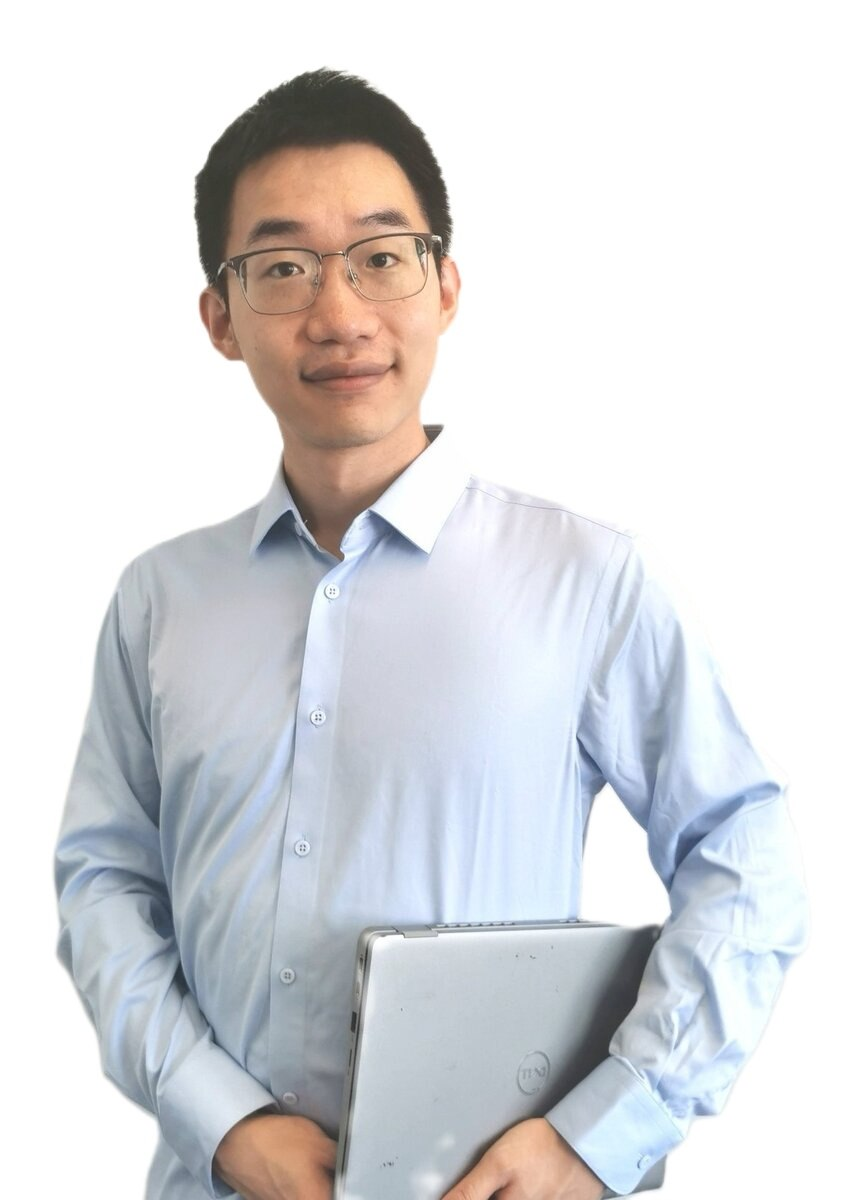
\includegraphics[
            width=0.65\textwidth,
            height=0.55\textheight,
            keepaspectratio
        ]{../zhongli-wang-profile.jpg}
    }{
        \vspace{0.55\textheight}
    }
\end{center}

\vspace{0.7cm}

% ---------- Personal Details ----------
\begin{center}
\renewcommand{\arraystretch}{1.35}
\begin{tabular}{>{\bfseries}p{4.2cm} p{8.5cm}}

Anschrift: & Astastrasse 22, 33617 Bielefeld, Deutschland \\

Telefon: & +49 160 9541 6015 \\

E-Mail: & nkwangzhongli@gmail.com \\

\end{tabular}
\end{center}

\vfill

\newpage
\enlargethispage{4\baselineskip}

\begin{flushright}
Zhongli Wang \\
Astastrasse 22 \\
33617 Bielefeld \\
Deutschland \\
\end{flushright}

\vspace{0.03cm}

\noindent
BKW Energie AG \\
z. Hd. Herrn Manrico Glauser \\
Head of Commodity Analysis

\vspace{0.15cm}

\noindent
\textbf{Bewerbung als Quantitative Commodity Analyst}

\vspace{0.15cm}

\noindent Sehr geehrter Herr Glauser,

ich bewerbe mich als Quantitative Commodity Analyst bei der BKW Energie AG. Ich promoviere derzeit in Wirtschaftswissenschaft an der Universität Bielefeld, mit geplanter Verteidigung am 21. September 2026, und besitze einen M.A. in Business and Economics mit Schwerpunkt Banking and Finance sowie einen B.Sc. in Finance. Meine quantitative Ausbildung in Modellierung, Datenanalyse und Preisprognose bildet eine solide Grundlage für die Entwicklung und Kalibrierung von Analysewerkzeugen für europäische Energiemärkte.

Die Verbindung von quantitativer Modellierung, Datenanalyse und Handelsentscheidungen in dynamischen Märkten spricht mich besonders an. In meiner Promotion entwickle ich Python-basierte Modelle, kalibriere Parameter und untersuche strategische Entscheidungen und Marktdynamiken unter Unsicherheit. In einem veröffentlichten Projekt analysierte ich Finanz- und Marktdaten mit maschinellem Lernen (XGBoost, Random Forest) zur Risikoidentifikation. Dabei habe ich gelernt, Modelle zu implementieren, ihre Performance zu überwachen, Annahmen zu validieren und komplexe Analyseergebnisse verständlich zu kommunizieren.

Für Ihr Analyseteam bringe ich insbesondere mit:

\begin{itemize}
    \item fundierte Data-Science- und Modellierungskenntnisse mit praktischer Umsetzungserfahrung in Python (NumPy, pandas, scikit-learn), R, Julia und SQL-Datenbanken;
    \item Erfahrung in Modellentwicklung, Parameterkalibrierung, Backtesting und Performance-Überwachung quantitativer Modelle;
    \item ausgeprägte analytische Fähigkeiten, strukturierte Arbeitsweise und die Fähigkeit, komplexe Inhalte verständlich zu vermitteln;
    \item sehr gute Deutsch- und Englischkenntnisse sowie internationale Teamarbeitserfahrung.
\end{itemize}

Meine quantitative Ausbildung, kombiniert mit hoher Lernfähigkeit und Motivation, bietet eine solide Grundlage, um mich zügig in Strommärkte, Handelspositionen und die ökonomischen Zusammenhänge europäischer Energiemärkte einzuarbeiten. Ich bin motiviert, meine Modellierungs- und Programmiererfahrung auf Preisprognosemodelle und Handelsanalysen anzuwenden.

Mein frühestmöglicher Eintrittstermin ist nach Absprache. Über die Möglichkeit, meine quantitative Arbeitsweise und analytischen Fähigkeiten in Ihr dynamisches Analyseteam in Bern einzubringen und zum Handelserfolg der BKW beizutragen, würde ich mich sehr freuen.

Vielen Dank für Ihre Zeit und die Prüfung meiner Bewerbung! Ich freue mich auf die Gelegenheit, meine Motivation und meinen möglichen Beitrag zur BKW persönlich zu erläutern.

\vspace{0.1cm}
\noindent Mit freundlichen Grü\ss{}en, \\
\noindent Zhongli Wang

\vspace{-0.02cm}
\IfFileExists{../Wang-sig.jpg}{
\includegraphics[width=2.25cm,keepaspectratio]{../Wang-sig.jpg}}{}

\end{document}
